\subsection{Graphical workflow editor: \grappa}
\label{subsec:grappa}
Most of the time complex data analysis tasks cannot be solved by only applying a
single operator to the data. Rather, selections of various operators need to be
combined into more sophisticated {\em workflows} to extract desired result data.
\alida inherently supports the development of such workflows. On the programmatic level it provides extensions of the operator concept 
towards workflow objects, and on the user side it includes {\em Grappa}, {\em the} {\bf \em Grap}{\em hical} {\bf \em P}{\em rogramming} 
{\em Editor for} {\bf \em A}{\em lida}. Grappa allows for designing and manipulating workflows via graph edit operations, hence, offers 
an intuitive interface and large flexibility for developing workflows.

A workflow in \alida is defined as a graph data structure. Each node of the graph represents an \alida operator, while edges between 
different nodes encode the flow of data and control. Each node owns a selection of input and output ports which are associated with the
operator's parameters. Consequently, edges are directed, i.e., an edge always
connects an output port of one operator node with an input port of another. Grappa visualizes such workflow graphs and supports manual editing, manipulation, and also workflow execution
and analysis of results.

\begin{center}
\begin{figure}[t]
\begin{center}
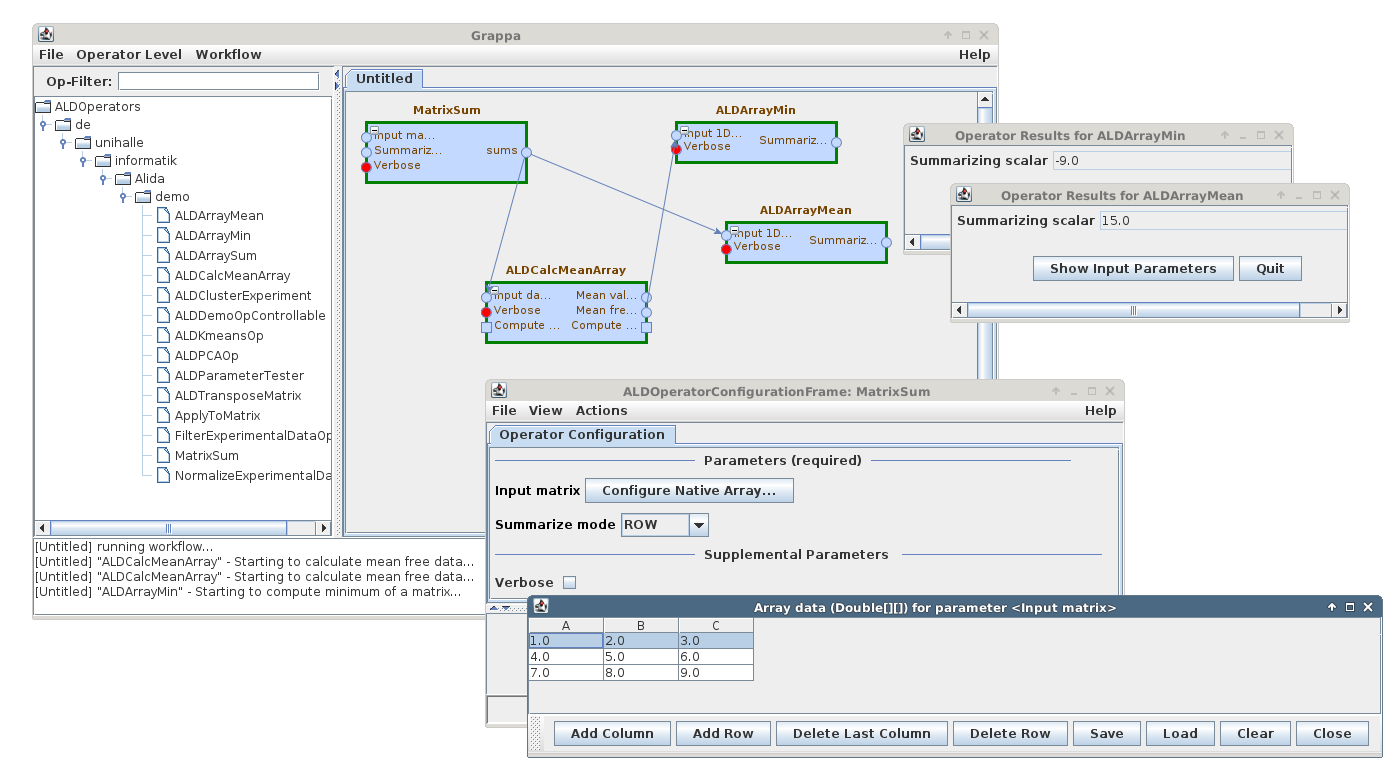
\includegraphics[width=0.975\textwidth,clip,trim = 15 20 10 10]
				{../images/screenShotGrappa.png}
\caption{\label{fig:grappaShot}Screenshot of the graphical editor {\em Grappa}.
In addition to the editor's main window (top left) two configuration windows for
data input (bottom) and two operator result frames (top right) are displayed.}
\end{center}
\end{figure}
\end{center}

\vspace*{-0.75cm}
Grappa can be started using the following command:
\vspace*{0.5cm}
\begin{code}
java de.unihalle.informatik.Alida.tools.ALDGrappaRunner
\end{code}

\vspace*{-0.25cm}
Figure \ref{fig:grappaShot} shows a screenshot of Grappa's main window. It is
basically divided into two sections. On the left, the node selection menu is
visible, while on the right the workbench area is located. 
In addition, the window features a menubar for configuring Grappa, loading and
saving workflows, and accessing the online help. At the bottom of the window a
panel displaying status and progress messages is available.

\subsubsection{Operator node selection menu} 
In the selection menu on the left of Grappa's main window all \alida operators found in the 
classpath upon initialization are listed as potential nodes for Grappa workflows. 
In analogy to the graphical user interface
 (see Sec.~\ref{subsec:userGUI}) they are arranged in a hierarchical ordering 
according to their package structure. The different package subtrees can be
folded and unfolded by double-clicking on a folder's name in the selection tree,
or by single-clicking on the circle displayed left to the folder icon. Above the
tree view an operator filter is available which allows to select operators
according to their names. For filtering, enter a substring into the text
field and press the return key. As for the graphical user interface, \alida
allows to customize the set of unfolded operators upon start-up to the user's needs
%To this end, the environment variable 
%{\tt ALIDA\_OPRUNNER\_FAVORITEOPS} needs to be set to a proper value, please 
(refer to Sec.~\ref{subsec:configure-user} for details). 
Operator nodes can be added to a workflow by double-clicking on the operator
name. A new operator node is then instantiated in the top left corner of the
corresponding workflow tab, i.e., the {\em active} workflow (see below).
Alternatively, an operator can be selected by clicking once on its name 
and afterwards clicking once on the position in the workflow tab where the new
operator node should be positioned.
 
\subsubsection{Workbench area} 
Workflows can be designed and executed in the workbench area on the right of the main window. It allows for instantiating
multiple workflows in parallel where each workflow is linked to an individual tab of the workbench panel. 
A new workflow tab can be added via the item {\tt 'New'} in the context menu of the workbench. 
The context menu is displayed upon right-click on an empty location of the workbench area. 
Upon selecting the item {\tt 'New'} a new tab is added to the workbench panel.
By default, the name of the new workflow is 'Untitled', but it can easily be
renamed via the corresponding item {\tt 'Rename'} in the context menu. Via this
menu it is also possible to close a workflow tab if no longer required. Note
that its contents are lost if not saved before! The currently selected tab in
the workbench contains the {\em active} workflow which can be edited and where
new operator nodes can be added as outlined in the previous subsection.

\paragraph{Operator nodes.} For each operator selected via the selection menu, a
node in terms of a rectangle is added to the currently active workflow. Above the rectangle 
the name of the operator is displayed, while on its left and right side the operator's input and output ports are shown as circles and 
squares. Circles are associated with operator parameters of directions {\tt IN} or {\tt OUT}, while squares refer to parameters with
direction {\tt INOUT} (Sec.~\ref{subsubsec:implOperators-basics}). The latter ports are duplicated on both sides of the node.
The colors of the circles indicate their type. Blue circles refer to required parameters, yellow circles are associated with optional 
parameters, and red circles are linked to supplemental parameters. To the left and right of the ports,
respectively, the name of the corresponding parameters are written.  
Once operator nodes have been added to a workflow, they can easily be dragged
and repositioned as well as resized via intuitive mouse actions. 

For each operator node a context menu can be popped up by clicking the node with the right mouse
button. From this menu it is possible to delete the node (item {\tt 'Remove'}), or to configure the
view via the item \icode{'Options'}. It, e.g., allows to select the set of operator parameter ports
to be shown, i.e.~either all parameters or just the subset of non-expert parameters. From the
context menu of a node it is also possible to configure the node (item {\tt 'Configure'}).  
\paragraph{Node configuration and states.} On selecting the item for
configuration, a window is displayed which allows to enter parameter values
(for an example, see the two windows at the bottom of Fig.~\ref{fig:grappaShot}).
The window is automatically generated, i.e., actually the same 
mechanisms as for executing operators via the graphical operator runner are applied (cf.~Sec.~\ref{subsec:userGUI}). Accordingly, 
the configuration window is identical to the corresponding operator control
window and shares the same layout, except for the control buttons and the batch
mode tab which are missing.

Operator parameters for a certain node can directly be specified via the
configuration window, they can be loaded from a proper parameter file in XML
format\footnote{The parameters of an operator can be saved to such a file via
the corresponding options in operator control windows as displayed by the
graphical operator runner. Also the node configuration windows in Grappa
provide an option to save the current parameter settings of the node.}, or they
can be configured by dragging edges between ports of different nodes with the
mouse to propagate output data from one node as input data to another. To add an
edge, move the mouse over an output port of a node until the port is surrounded
by a green square, then press the left mouse button. Subsequently, while keeping
the button pressed, move the mouse to the desired input port of another node.
Once a green rectangle shows up around the target input port, release the
button. Note that on dragging edges Grappa performs type and validity checks.
Only ports being associated with compatible parameter data types can be
linked to each other. Two parameter data types are compatible if they are
either equal, the target data type is a super class of the source data type, or
if \alida has access to a converter allowing to transform the source data type
into the target type (refer to Sec.~\ref{subsec:converter} for details). Also
edges are forbidden that would induce cycles into the workflow graph.

Nodes in a workflow can have different states indicated by the color of their border. 
Red framed nodes are not ready for execution, i.e., their configuration is not
complete. If a node is readily configured and can directly be executed, its
border has a yellow color, while nodes that are configured, however, require
additional input data from preceeding operator nodes have an orange color.
Prior to executing these orange nodes it is, thus, necessary to execute the
preceeding nodes first.
Note that Grappa takes care of such dependencies, i.e., automatically executes
nodes first from which result data is required for proper workflow or node
execution. The state of a node is updated by Grappa in real-time, i.e., each
change in its configuration directly invokes internal checkings and may result in a change of the node's color.

\paragraph{Workflow execution.} Grappa offers various modes for executing a
complete workflow or parts of it.
From the context menu of the workbench the item 
{\tt 'Run'} is available which executes the complete workflow, i.e., all nodes
currently present on the tab. From the context menu of a single node and its {\tt 'Run\ldots'} item also the whole workflow can be executed (item {\tt 'Workflow'}).
Alternatively, via the item {\tt 'Nodes from here'} it is possible to only execute the nodes of the workflow subgraph for which the 
current node is the root (of course considering required dependencies). Finally, the item {\tt 'Node'} allows for running the workflow
until the node in question. As mentioned before, Grappa automatically takes care
of resolving dependencies, i.e., upon executing a node all nodes having a yellow
or orange border and being predecessors of the node in question are also executed. Note that the execution of a workflow will fail if one of the nodes is still colored red, or if a node does not produce proper output data required by others. 

After successful execution of the workflow or a subset of nodes, the colors of
the corresponding nodes change to green indicating that result data are
available. For all terminal nodes having no successor the result frames are
automatically opened (see Fig.~\ref{fig:grappaShot} top right).
For all other nodes the result data can graphically be examined via the nodes'
context menus from which the result windows can manually be opened. 
Once a node has been executed and is colored in green, it is not possible to
re-execute the node until its configuration, or at least the configuration of
one of its preceeding nodes, was changed.

\subsubsection{Menubar and shortcuts} The Grappa main window features a menubar offering quick
access to the basic functions of Grappa and some additional convenience functionality simplifying
the work with the editor. 

Via the menu item \icode{'File'} workflows can be saved to and read from
disk. By saving a workflow currently two files are written to disk, one containing the information
about the nodes and their configuration, and one storing graphical information
regarding the current workflow layout. Both are required to load a workflow
again. The first one has the extension \icode{'.awf'}, the latter one the
extension \icode{'.awf.gui'}.

Via the menu item {\tt 'Workflow'} new workflows can be added and existing ones be renamed, 
closed, executed or interrupted.  
As outlined in Sec.~\ref{subsec:userGUI}, \alida supports two categories of
operators, i.e.~operators mainly dedicated to direct application by non-expert users
and operators for special tasks and expert usage. Via the item \icode{'Options'} the menubar allows
to switch the view in the selection menu between both categories. Also progress messages triggered by the
operator node during execution and optionally shown in the status panel can be enabled or
disabled via this menu. Finally, the menu item {\tt 'Help'} grants access to \alida's online help system
where information about its functionality and descriptions of the operators can be found.

The most important functions for workflow and node handling in Grappa are also
accessible via keyboard shortcuts. Currently the following shortcuts are
implemented:
\begin{itemize} 
  \item \icode{Ctrl-N} \hspace*{0.5cm} --- \hspace*{0.5cm}
  	open a new, empty workflow in a new tab
  \item \icode{Ctrl-U} \hspace*{0.5cm} --- \hspace*{0.5cm}
  	rename the active workflow
  \item \icode{Ctrl-W} \hspace*{0.5cm} --- \hspace*{0.5cm}
  	close the active workflow
  \item \icode{Ctrl-S} \hspace*{0.5cm} --- \hspace*{0.5cm}
	save the active workflow to disk
  \item \icode{Ctrl-L} \hspace*{0.5cm} --- \hspace*{0.5cm}
  	load a workflow from disk into a new tab
  \item \icode{Ctrl-A} \hspace*{0.5cm} --- \hspace*{0.5cm}
	run the complete workflow
  \item \icode{Ctrl-P} \hspace*{0.5cm} --- \hspace*{0.5cm} 
	open the configuration frames of all selected nodes in the active workflow
  \item \icode{Ctrl-X} \hspace*{0.5cm} --- \hspace*{0.5cm}
	delete all selected nodes in the active workflow
\end{itemize}
